\chapter{Background}\label{chap:background}

Hardware security sits at the intersection of physical engineering and adversarial thinking. While software vulnerabilities dominate public attention, a growing body of research demonstrates that physical access to a device often collapses its entire security model---authentication bypassed through a serial console, encryption rendered irrelevant by reading plaintext flash, firmware integrity undermined by the absence of secure boot. We introduce the foundational concepts that the rest of this thesis builds upon: the threat landscape, the architecture of the embedded systems we target, the protocols through which they can be interrogated, and the tools that make analysis practical. Throughout, we use the TP-Link WR841N router---the case study device of Chapter~\ref{chap:casestudy}---as a running example.

% ============================================================================
\section{Foundations of Hardware Security}\label{sec:hw-security}
% ============================================================================

\subsection{The Role of Hardware in Cybersecurity}\label{subsec:hw-role}

Software-centric security models rest on an implicit assumption: the underlying hardware operates correctly and cannot be tampered with. Physical access invalidates this assumption. An adversary who can touch a device can probe electrical signals, read flash memory, inject faults, or extract cryptographic keys through side-channel observations~\cite{anderson2020security}. Hardware is therefore both the foundation of all software security guarantees and, when inadequately protected, a direct path to compromise.

Prinetto~\cite{prinetto2019hardware} classifies hardware security threats along three dimensions: abstraction level (circuit, microarchitecture, system), required access (remote, local, physical), and outcome (information leakage, denial of service, control hijack). The classification underscores that hardware security is not a single discipline but a family of concerns---a fact reflected in the breadth of the training objectives we define for the \pcbctf{} platform.

\subsection{Hardware Security Threats and Adversary Motivations}\label{subsec:hw-threats}

Adversary motivations span intellectual property theft, espionage, sabotage, and financially motivated attacks---most notably against consumer IoT devices, where low cost, minimal security investment, and massive deployment volumes converge into an especially attractive target profile~\cite{becker2013stealthy, antonakakis2017mirai}.

The attack vectors most relevant to this work are:
\begin{itemize}
    \item \textbf{Debug interface exploitation.} Protocols such as UART, JTAG, and SWD left accessible on production boards provide direct console access or memory read-out~\cite{shwartz2017}. On the WR841N, the UART header yields an unauthenticated root shell.
    \item \textbf{Firmware extraction and analysis.} Flash contents read via SPI or I\textsuperscript{2}C expose filesystem images, cryptographic keys, and hardcoded credentials~\cite{costin2014large}. The WR841N's Winbond W25Q32 NOR flash chip can be dumped with a \$5 CH341A programmer.
    \item \textbf{Side-channel analysis.} Power consumption, electromagnetic emissions, and timing variations during cryptographic operations can reveal secret key material~\cite{kocher1999dpa}.
    \item \textbf{Fault injection.} Voltage glitching, clock manipulation, or laser illumination can alter execution flow, bypassing security checks or corrupting cryptographic computations~\cite{barenghi2012fault}.
\end{itemize}

The first two vectors---debug interfaces and firmware extraction---are the focus of the \pcbctf{} platform, because they represent the entry-level skills most frequently exercised in professional hardware security assessments and are amenable to faithful browser-based simulation.

\subsection{Hardware Analysis Methodology}\label{subsec:hw-compromise}\label{subsec:methodology}

Hardware compromise follows a structured methodology that experienced analysts apply almost instinctively but that students must learn through deliberate practice. The workflow proceeds in seven phases, illustrated in Figure~\ref{fig:hw-methodology}:

\begin{enumerate}
    \item \textbf{Physical reconnaissance.} The analyst opens the device enclosure and inspects the PCB, identifying major ICs (SoC, flash, DRAM), connectors, test points, and component markings. On the WR841N, this step immediately reveals the QCA9533 SoC (the largest BGA package on the board), the Winbond W25Q32 flash chip (8-pin SOIC near the SoC), and a row of four through-holes near the board edge that suggest a UART header.

    \item \textbf{Electrical characterisation.} The analyst measures voltage levels and impedances at suspected interface pins using a multimeter. On the WR841N UART header, pin~1 reads 3.3\,V with low impedance ($\sim$65\,$\Omega$, identifying it as TX), pin~2 reads 3.3\,V with high impedance ($\sim$47\,k$\Omega$, identifying it as RX), pin~3 reads 0\,V (GND), and pin~4 reads 3.3\,V (VCC, unused for communication).

    \item \textbf{Interface identification.} Based on the electrical measurements, the analyst confirms the protocol type and pin assignments. Three wires at 3.3\,V/0\,V levels with the described impedance pattern is a strong UART signature.

    \item \textbf{Communication establishment.} The analyst connects a USB-to-Serial adapter with correct crossover wiring (adapter TX to device RX, adapter RX to device TX, GND to GND) and opens a terminal emulator at 115\,200\,bps.

    \item \textbf{Firmware extraction.} For devices with SPI flash, the analyst connects a flash programmer (e.g., CH341A) to the chip's VCC, GND, CS, CLK, MOSI, and MISO pins and reads the full flash contents to a binary file.

    \item \textbf{Firmware analysis.} The extracted binary is processed with Binwalk to identify and extract filesystem images. The root filesystem is mounted and explored for configuration files, credentials, and executables of interest.

    \item \textbf{Vulnerability identification.} The analyst searches for hardcoded credentials (in files such as \texttt{/etc/shadow} and \texttt{/etc/passwd}), sensitive data in configuration partitions (via \texttt{strings} on raw partition images), and vulnerable code patterns in binaries (e.g., injection-prone function calls found with~\texttt{strings}).
\end{enumerate}

This progression forms the pedagogical backbone of the \pcbctf{} platform, where each phase maps to one or more exercise objectives. The platform cannot fully replicate the physical experience of holding a probe against a test pad, but it faithfully reproduces the \emph{reasoning process}: observe, measure, hypothesise, connect, extract, analyse. The case study in Chapter~\ref{chap:casestudy} demonstrates that this reasoning process can be taught effectively through simulation.

\begin{figure}[ht]
    \centering
    \begin{tikzpicture}[
        node distance=0.6cm,
        box/.style={rectangle, draw, fill=blue!8, minimum width=4.2cm, minimum height=0.8cm, align=center, font=\small},
        arr/.style={-{Stealth[length=2.5mm]}, thick, shorten >=2pt, shorten <=2pt}
    ]
    \node[box] (n1) {1. Physical Reconnaissance};
    \node[box, below=of n1] (n2) {2. Electrical Characterisation};
    \node[box, below=of n2] (n3) {3. Interface Identification};
    \node[box, below=of n3] (n4) {4. Communication Establishment};
    \node[box, below=of n4] (n5) {5. Firmware Extraction};
    \node[box, below=of n5] (n6) {6. Firmware Analysis};
    \node[box, below=of n6] (n7) {7. Vulnerability Discovery};
    \foreach \i/\j in {n1/n2, n2/n3, n3/n4, n4/n5, n5/n6, n6/n7}
        \draw[arr] (\i) -- (\j);
    \end{tikzpicture}
    \caption{Overview of the hardware analysis methodology. Each phase maps to one or more exercise objectives in the \pcbctf{} platform.}
    \label{fig:hw-methodology}
\end{figure}

% ============================================================================
\section{Embedded Systems Fundamentals}\label{sec:embedded}
% ============================================================================

\subsection{Architecture of Consumer IoT Devices}\label{subsec:embedded-def}

The WR841N exemplifies the architecture common to the vast majority of consumer IoT devices: a System-on-Chip (SoC) integrating CPU core, memory controllers, and peripheral interfaces; a NOR flash chip for non-volatile storage; DRAM for runtime memory; and a PCB that interconnects these components through copper traces. The SoC---in this case the Qualcomm Atheros QCA9533, a MIPS-based processor clocked at 650\,MHz---is typically the largest IC on the board and can be identified visually by package size and pin count.

\subsection{Common SoC Families and Components}\label{subsec:embedded-components}

Beyond the QCA95xx series found in TP-Link routers, common SoC families in low-cost IoT devices include MediaTek MT76xx (routers and access points) and Realtek RTL8196/RTL8197 (networking equipment). These processors run MIPS or ARM cores at 400\,MHz to 1\,GHz, with 32--128\,MB of DRAM and 4--32\,MB of flash. The WR841N sits at the lower end of this spectrum: 4\,MB NOR flash (Winbond W25Q32, 8-pin SOIC package) and 32\,MB DRAM---enough to run a stripped-down Linux distribution but with no margin for encryption overhead or integrity checking, a trade-off with direct security consequences.

\begin{figure}[ht]
    \centering
    \begin{tikzpicture}[
        block/.style={rectangle, draw, fill=blue!8, minimum width=2.4cm, minimum height=1cm, align=center, font=\small},
        soc/.style={rectangle, draw, fill=orange!12, minimum width=3.8cm, minimum height=2.2cm, align=center, font=\small\bfseries},
        iface/.style={rectangle, draw, fill=green!10, minimum width=1.8cm, minimum height=0.7cm, align=center, font=\footnotesize},
        arr/.style={-{Stealth[length=2.5mm]}, thick, shorten >=2pt, shorten <=2pt},
        darr/.style={{Stealth[length=2.5mm]}-{Stealth[length=2.5mm]}, thick, shorten >=2pt, shorten <=2pt}
    ]
    \node[soc] (soc) {SoC\\{\footnotesize (CPU + Peripherals)}};
    \node[block, right=2cm of soc] (flash) {NOR Flash\\{\footnotesize 4--32\,MB}};
    \node[block, left=2cm of soc] (dram) {DRAM\\{\footnotesize 32--128\,MB}};
    \node[iface, below left=1.2cm and 0.3cm of soc] (uart) {UART};
    \node[iface, below=1.2cm of soc] (spi) {SPI};
    \node[iface, below right=1.2cm and 0.3cm of soc] (jtag) {JTAG};
    \draw[darr] (soc) -- node[above, font=\footnotesize]{SPI bus} (flash);
    \draw[darr] (soc) -- node[above, font=\footnotesize]{data bus} (dram);
    \draw[arr] (soc) -- (uart);
    \draw[arr] (soc) -- (spi);
    \draw[arr] (soc) -- (jtag);
    \end{tikzpicture}
    \caption{Block diagram of a typical consumer-grade embedded system, showing the SoC, flash memory, DRAM, and debug interfaces (UART, SPI, JTAG).}
    \label{fig:embedded-block}
\end{figure}

\subsection{Non-Volatile Storage and Flash Layout}\label{subsec:storage}

Consumer IoT devices overwhelmingly use NOR flash for firmware storage, accessed via SPI. NOR flash provides random read access---essential for execute-in-place bootloaders---and ships in compact 8-pin SOIC packages that are straightforward to probe with clip adapters. Higher-density NAND flash appears in devices with larger storage needs but requires a flash translation layer for wear levelling. EEPROM, with byte-level write granularity, is occasionally used for small configuration blobs.

On the WR841N and similar devices, the entire firmware---bootloader, kernel, and root filesystem---resides on a single NOR flash chip. The typical partition layout, shown in Figure~\ref{fig:flash-layout}, dedicates the first sector to U-Boot, followed by the compressed kernel, a read-only SquashFS root filesystem, and a writable JFFS2 configuration partition.

\begin{figure}[ht]
    \centering
    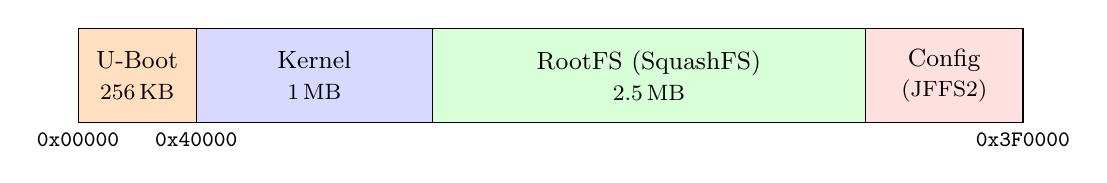
\begin{tikzpicture}[font=\small]
    \def\totalw{12}
    % Partition widths (proportional to typical sizes)
    \def\bw{1.5}   % bootloader 256KB
    \def\kw{3.0}   % kernel 1MB
    \def\rw{5.5}   % rootfs 2.5MB
    \def\cw{2.0}   % config 256KB
    % Draw partitions
    \fill[orange!25] (0,0) rectangle (\bw,1.2);
    \draw (0,0) rectangle (\bw,1.2);
    \node[align=center] at (\bw/2, 0.6) {U-Boot\\{\footnotesize 256\,KB}};
    %
    \fill[blue!15] (\bw,0) rectangle (\bw+\kw,1.2);
    \draw (\bw,0) rectangle (\bw+\kw,1.2);
    \node[align=center] at (\bw+\kw/2, 0.6) {Kernel\\{\footnotesize 1\,MB}};
    %
    \fill[green!15] (\bw+\kw,0) rectangle (\bw+\kw+\rw,1.2);
    \draw (\bw+\kw,0) rectangle (\bw+\kw+\rw,1.2);
    \node[align=center] at (\bw+\kw+\rw/2, 0.6) {RootFS (SquashFS)\\{\footnotesize 2.5\,MB}};
    %
    \fill[red!12] (\bw+\kw+\rw,0) rectangle (\totalw,1.2);
    \draw (\bw+\kw+\rw,0) rectangle (\totalw,1.2);
    \node[align=center] at (\bw+\kw+\rw+\cw/2, 0.6) {Config\\{\footnotesize (JFFS2)}};
    % Offset labels
    \node[below, font=\footnotesize] at (0, 0) {\texttt{0x00000}};
    \node[below, font=\footnotesize] at (\bw, 0) {\texttt{0x40000}};
    \node[below, font=\footnotesize] at (\totalw, 0) {\texttt{0x3F0000}};
    \end{tikzpicture}
    \caption{Typical flash memory partition layout in a Linux-based IoT device, showing the bootloader, kernel, root filesystem (SquashFS), and configuration (JFFS2) partitions.}
    \label{fig:flash-layout}
\end{figure}

\subsection{MTD Subsystem}\label{subsec:mtd}

Linux-based embedded systems organise flash through the Memory Technology Device (MTD) subsystem, which exposes raw flash partitions as block devices (\texttt{/dev/mtdblockN}). The configuration partition in particular is of interest to an attacker: it frequently stores Wi-Fi credentials, PPPoE passwords, and administrative credentials in plaintext or with trivially reversible encoding.

\subsection{CPU Architectures}\label{subsec:cpu-arch}

ARM and MIPS dominate the IoT space---ARM in smartphones, wearables, and higher-end embedded devices, MIPS in networking equipment from TP-Link, D-Link, and Netgear. Knowing the target ISA determines the disassembly toolchain (Ghidra, IDA Pro), the calling conventions, and the exploitation techniques available to the analyst.

\subsection{U-Boot and the Boot Chain}\label{subsec:uboot}

Das U-Boot is the de facto standard bootloader for embedded Linux. It handles hardware initialisation, memory testing, and kernel loading from flash into RAM. A command-line interface, accessible via UART during a configurable timeout window, exposes commands that are invaluable for security analysis: \texttt{printenv} reveals boot arguments and memory layout, \texttt{md} dumps arbitrary memory regions, and \texttt{sf read/write} performs SPI flash operations. On the WR841N, \texttt{printenv} discloses the kernel load address, root filesystem type, and boot arguments---information that the \pcbctf{} case study exercise uses as the basis for its first terminal challenge.

\begin{figure}[ht]
    \centering
    \begin{tikzpicture}[
        node distance=0.3cm and 0.5cm,
        box/.style={rectangle, draw, fill=blue!8, minimum width=1.7cm, minimum height=0.7cm, align=center, font=\scriptsize},
        arr/.style={-{Stealth[length=2mm]}, thick, shorten >=2pt, shorten <=2pt}
    ]
    \node[box] (por) {Power-On\\Reset};
    \node[box, right=of por] (rom) {ROM\\Bootloader};
    \node[box, right=of rom] (uboot) {U-Boot\\Init};
    \node[box, right=of uboot] (kernel) {Kernel\\Load};
    \node[box, right=of kernel] (mount) {Mount\\RootFS};
    \node[box, right=of mount] (init) {\texttt{/sbin/init}};
    \foreach \i/\j in {por/rom, rom/uboot, uboot/kernel, kernel/mount, mount/init}
        \draw[arr] (\i) -- (\j);
    \end{tikzpicture}
    \caption{Boot chain of a typical embedded Linux device: power-on reset, ROM bootloader, U-Boot initialisation, kernel loading, root filesystem mount, and \texttt{init} process.}
    \label{fig:boot-chain}
\end{figure}

\subsection{RTOS vs.\ Linux-Based Systems}\label{subsec:rtos-linux}

Embedded devices split into two broad categories: Real-Time Operating Systems (FreeRTOS, Zephyr, proprietary firmware) and Linux-based distributions (typically OpenWrt or vendor-customised BusyBox). The latter---dominant in consumer routers and IP cameras---offers a familiar Unix environment that is more accessible to exploitation and constitutes the target category of the \pcbctf{} platform.

% ============================================================================
\section{Debug and Communication Interfaces}\label{sec:interfaces}
% ============================================================================

UART and SPI are the two serial protocols most relevant to this work, as they constitute the primary interfaces through which the \pcbctf{} platform simulates hardware interaction.

\subsection{UART}\label{subsec:uart-protocol}

The Universal Asynchronous Receiver-Transmitter is a point-to-point serial protocol used extensively for debug consoles. Without a shared clock, both endpoints must agree on a baud rate---115\,200\,bps is standard for embedded consoles. Each frame consists of a start bit (logic low), 8 data bits (LSB first), an optional parity bit, and one or two stop bits (logic high).

A minimal connection requires three wires: TX, RX, and GND. The critical wiring rule is the \emph{crossover convention}: the TX output of one device connects to the RX input of the other. The \pcbctf{} platform explicitly validates this rule during the UART connection step (Section~\ref{subsec:uart-impl}).

\begin{figure}[ht]
    \centering
    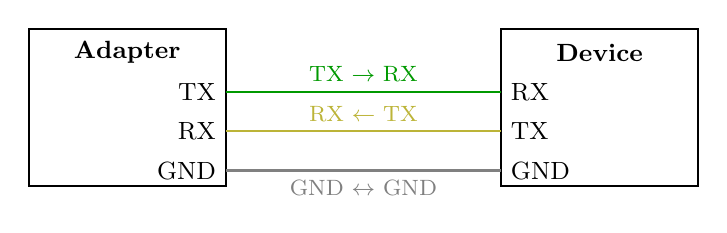
\begin{tikzpicture}[font=\small]
    % Device A
    \draw[thick] (0,0.3) rectangle (2.5, 2.3);
    \node[font=\small\bfseries] at (1.25, 2.0) {Adapter};
    \node[anchor=east] at (2.5, 1.5) {TX};
    \node[anchor=east] at (2.5, 1.0) {RX};
    \node[anchor=east] at (2.5, 0.5) {GND};
    % Device B
    \draw[thick] (6,0.3) rectangle (8.5, 2.3);
    \node[font=\small\bfseries] at (7.25, 2.0) {Device};
    \node[anchor=west] at (6, 1.5) {RX};
    \node[anchor=west] at (6, 1.0) {TX};
    \node[anchor=west] at (6, 0.5) {GND};
    % Crossover wires
    \draw[thick, green!60!black] (2.5, 1.5) -- (6, 1.5);
    \draw[thick, yellow!70!black] (2.5, 1.0) -- (6, 1.0);
    \draw[thick, gray] (2.5, 0.5) -- (6, 0.5);
    % Labels
    \node[font=\footnotesize, green!60!black, above] at (4.25, 1.5) {TX $\to$ RX};
    \node[font=\footnotesize, yellow!70!black, above] at (4.25, 1.0) {RX $\leftarrow$ TX};
    \node[font=\footnotesize, gray, below] at (4.25, 0.5) {GND $\leftrightarrow$ GND};
    \end{tikzpicture}
    \caption{UART crossover wiring convention. The adapter's TX connects to the device's RX and vice versa. GND is shared directly.}
    \label{fig:uart-crossover}
\end{figure}

From a security standpoint, UART consoles matter because manufacturers routinely leave them enabled on production boards. On the WR841N, the four-pin header near the SoC provides an unauthenticated root shell at 115\,200\,bps---no password prompt, no rate limiting. Shwartz et al.~\cite{shwartz2017} found that over 45\% of analysed IoT devices exposed an active UART interface.

Identifying UART pins on an unknown board involves two steps: (i)~visual inspection for groups of 3--4 aligned pins near the SoC, and (ii)~multimeter measurement. TX idles at logic high (3.3\,V, low output impedance $\sim$65\,$\Omega$), RX also idles high but with high input impedance ($\sim$47\,k$\Omega$ due to a pull-up resistor), and GND reads 0\,V. These impedance differences allow an analyst to distinguish TX from RX without an oscilloscope---a technique the \pcbctf{} multimeter simulation reproduces.

\subsection{SPI}\label{subsec:spi-protocol}

The Serial Peripheral Interface is a synchronous, full-duplex protocol used primarily for flash memory access. It uses four signals: CS (Chip Select, active low) selects the target peripheral; CLK (Clock) synchronises transfers; MOSI (Master Out, Slave In) carries data to the peripheral; MISO (Master In, Slave Out) carries data back. VCC and GND complete the connection.

For firmware extraction, a flash programmer such as the CH341A acts as SPI master, issuing read commands over MOSI and capturing responses on MISO. The \pcbctf{} platform simulates this by requiring six correct probe connections (VCC, GND, CS, CLK, MOSI, MISO) before initiating the dump.

In idle state (CS deasserted), the SPI signals exhibit characteristic voltage levels: CS is pulled high to 3.3\,V via a 10\,k$\Omega$ pull-up; CLK and MOSI are driven low by the SoC ($\sim$65\,$\Omega$ output impedance); MISO floats at $\sim$0.15\,V with very high impedance ($\sim$150\,k$\Omega$) because the flash output is tri-stated when not selected. These signatures guide pin identification and are reproduced in the platform's multimeter simulation.

% ============================================================================
\section{Hardware and Software Tools}\label{sec:tools}
% ============================================================================

\subsection{Hardware Instrumentation}\label{subsec:hw-tools}

Embedded device analysis requires a modest toolkit:
\begin{itemize}
    \item \textbf{Digital multimeter.} Identifies voltage levels on PCB test points---3.3\,V near the SoC may indicate a UART TX line, 0\,V indicates ground.
    \item \textbf{USB-to-Serial adapter.} Converts UART signals to USB for serial console access. FTDI FT232 and CP2102 adapters are standard.
    \item \textbf{Logic analyser.} Captures digital signals on multiple channels for protocol identification and timing analysis.
    \item \textbf{SPI flash programmer.} The CH341A reads and writes flash memory chips directly, enabling firmware extraction without powering the target device.
\end{itemize}

\subsection{Software Toolchain}\label{subsec:sw-tools}

After firmware extraction, analysis proceeds with:
\begin{itemize}
    \item \textbf{Binwalk}~\cite{binwalk}: scans binary images for file signatures and entropy patterns, automating filesystem extraction.
    \item \textbf{Flashrom}~\cite{flashrom}: reads, writes, and verifies flash chips via SPI, parallel, or FWH interfaces.
    \item \textbf{Ghidra}~\cite{ghidra}: supports disassembly and decompilation for ARM, MIPS, and other architectures.
    \item \textbf{Hashcat / John the Ripper}: recover cleartext passwords from hashes extracted from \texttt{/etc/shadow} or configuration files.
    \item \textbf{Strings}: extracts printable character sequences from binary files, often revealing hardcoded credentials and debug messages.
\end{itemize}

\subsection{Exploitability Factors in Consumer IoT Devices}\label{subsec:exploitability}

The vulnerabilities encountered during hardware analysis of consumer IoT devices are not random; they follow recurring patterns rooted in economic and engineering trade-offs. Understanding these patterns is essential for designing training exercises that cover the most practically relevant attack categories. Based on the literature~\cite{shwartz2017, costin2014large, genova2025} and the device analyses informing the case study in Chapter~\ref{chap:casestudy}, we identify six key exploitability factors---each of which maps to a specific training objective in the \pcbctf{} platform:

\begin{enumerate}
    \item \textbf{Exposed debug interfaces.} UART headers, JTAG test points, and SWD connectors are frequently left accessible on production boards. Manufacturers include them for factory testing and field diagnostics but rarely disable them before shipping~\cite{shwartz2017}. \emph{Training objective:} the platform teaches students to visually locate these headers and verify them with multimeter measurements before establishing a serial connection---the core skill exercised in the UART connection step.

    \item \textbf{Unencrypted firmware storage.} SPI NOR flash contents are stored in plaintext, with no encryption or integrity verification. The entire firmware of the WR841N can be read with a CH341A programmer in under 30 seconds. \emph{Training objective:} the SPI firmware dump step requires students to correctly identify and connect all six probe wires, reinforcing the physical extraction workflow.

    \item \textbf{Hardcoded credentials.} Default passwords for administrative access are embedded in the firmware and are often identical across all units of a given model. On the WR841N, the credentials \texttt{root}/\texttt{sohoadmin} are widely documented. \emph{Training objective:} a terminal challenge requires the student to gain root access using these default credentials, demonstrating why hardcoded passwords are a systemic risk.

    \item \textbf{Sensitive data in configuration partitions.} The JFFS2 configuration partition on many routers stores Wi-Fi passwords, PPPoE credentials, and administrative passwords in plaintext or with trivially reversible encoding. Running \texttt{strings} on the raw partition image is often sufficient. \emph{Training objective:} a terminal challenge tasks the student with extracting credentials from the configuration partition, reinforcing both the \texttt{strings} technique and the MTD partition model.

    \item \textbf{Absent secure boot.} Most low-cost IoT devices lack a hardware root of trust. The bootloader does not verify kernel integrity or authenticity, enabling firmware modification attacks. \emph{Training objective:} the U-Boot analysis challenge asks the student to identify inconsistencies in boot environment variables that reveal the absence of integrity checking.

    \item \textbf{Vulnerable network services.} Web servers and UPnP services on IoT devices frequently contain command injection vulnerabilities---functions like \texttt{execFormatCmd()} or direct \texttt{system()} calls with unsanitised input are common findings. \emph{Training objective:} a binary analysis challenge in the terminal phase requires the student to locate such a vulnerable function in the extracted firmware, connecting the hardware extraction workflow to its ultimate security payoff.
\end{enumerate}

% ============================================================================
\section{Web Technologies and Frameworks}\label{sec:web-frameworks}
% ============================================================================

The \pcbctf{} platform is not only a hardware security training tool: it is also a modern single-page web application whose design decisions---client-side simulation, zero-install deployment, declarative authoring---depend critically on a specific ecosystem of web technologies. This section introduces, at a foundational level, the families of frameworks and patterns that together constitute that ecosystem. Our goal is to equip the reader with enough vocabulary to follow the architectural discussion in Chapter~\ref{chap:architecture} and the implementation details in Chapter~\ref{chap:implementation}, where the specific choices adopted by \pcbctf{} are motivated and put into practice.

\subsection{Modern Web Application Architectures}\label{subsec:web-architectures}

Web applications have historically oscillated between two rendering models. In the \emph{multi-page} model, every user navigation triggers a full round trip to the server, which returns a complete HTML document; this approach is simple and search-engine friendly but produces perceived latency on every interaction. The \emph{single-page application} (SPA) model, popularised in the early 2010s, loads a JavaScript bundle once and performs subsequent navigation and data fetching entirely on the client, yielding near-instant interactions at the cost of longer initial loads and more complex state management.

Contemporary \emph{meta-frameworks} attempt to combine the strengths of both approaches. They support \emph{server-side rendering} (SSR) or \emph{static site generation} (SSG) to produce pre-rendered HTML for the first paint, then \emph{hydrate} the document on the client so that subsequent interactions behave as in an SPA. \nextjs{}~\cite{nextjs} is a representative example: built on top of \reactjs{} (Section~\ref{subsec:react-components}), it introduces a file-system-based routing scheme, hybrid rendering modes selectable per route, and---in recent versions---a \emph{standalone output} mode that produces a self-contained Node.js server image suitable for single-container deployment. These capabilities are what allow a simulator like \pcbctf{} to ship as a single Docker artifact while still offering SPA-like interactivity.

\subsection{Component-Based UI Development with React}\label{subsec:react-components}

\reactjs{}~\cite{reactdocs} is a JavaScript library for building user interfaces based on a \emph{component} abstraction: the interface is decomposed into self-contained, reusable units, each of which declaratively describes its rendered output as a function of its current inputs. Rather than mutating the Document Object Model (DOM) directly, React maintains an in-memory representation---the \emph{virtual DOM}---and computes a minimal set of DOM operations through a diffing algorithm called reconciliation. This separation between the declared state and the physical DOM is what allows complex, deeply nested interfaces to update efficiently in response to state changes.

Since the introduction of \emph{hooks} in React~16.8, function components (as opposed to the older class-based components) have become the idiomatic unit of UI code. Hooks such as \texttt{useState}, \texttt{useEffect}, and \texttt{useRef} let function components encapsulate local state, side effects, and mutable references without inheritance. The declarative, composable style that hooks encourage maps naturally onto the kind of richly interactive UI required by a hardware simulator, where probes, overlays, and terminal tabs all need to react to a shared underlying state in a predictable way.

\subsection{Static Typing in JavaScript Ecosystems}\label{subsec:typescript-bg}

JavaScript is a dynamically typed language, which is well suited to rapid prototyping but increasingly fragile as a codebase grows. \typescript{}~\cite{typescripthandbook} addresses this limitation by layering a \emph{structural} type system on top of JavaScript: any valid JavaScript program is also a valid TypeScript program, and type annotations are erased at compile time to produce plain JavaScript output. The typing discipline is structural rather than nominal---two types are considered compatible if their shapes match, regardless of their declared names---which aligns well with the duck-typed idioms of existing JavaScript libraries.

TypeScript supports \emph{gradual} adoption: individual files, or even individual variables within a file, may remain untyped, enabling incremental migration of legacy code. In modern React projects, however, strict compiler settings (\texttt{strict}, \texttt{noImplicitAny}, \texttt{strictNullChecks}) are increasingly the default, and the type system is used to encode invariants such as exhaustive handling of enumerated message types, nullable reference tracking, and discriminated unions for state machines. For a domain with as many moving parts as a hardware simulator, this form of compile-time verification shortens the feedback loop on refactors and reduces the surface for regressions.

\subsection{Client-Side State Management}\label{subsec:state-management}

As SPAs grew in complexity, the question of how to organise state that is shared between many components became a first-class architectural concern. An early and influential answer was the \emph{Flux} pattern proposed by Facebook, in which UI events are transformed into explicit \emph{actions} that flow through a central dispatcher and produce new immutable state in one or more stores. Redux~\cite{redux} popularised a refined version of this pattern, combining a single global store, pure reducer functions, and time-travel debugging tools.

Flux/Redux promotes predictability at the cost of considerable boilerplate: defining actions, action creators, reducers, and selectors for every slice of state. In response, a second generation of state libraries has emphasised ergonomics. \zustand{}~\cite{zustand} is representative: it exposes a minimalist API in which a store is a plain function returning state and actions, components subscribe through a single hook, and updates are triggered by direct function calls rather than dispatched actions. This lean approach retains the centralised-store benefits---shared state across components, easy persistence, clear ownership---while drastically reducing the amount of code required. Such lightweight stores are particularly well suited to applications like a PCB simulator, in which multiple specialised stores (e.g.\ one for exercise progress, one for authoring drafts, one for terminal configuration) must coexist without imposing a single monolithic state tree.

\subsection{Styling and Accessible UI Primitives}\label{subsec:styling-ui}

The styling layer of modern web applications has converged on a set of complementary practices in which utility-first CSS, accessible unstyled primitives, and source-level component distribution replace the monolithic design systems of earlier generations.

The \emph{utility-first} approach, popularised by \tailwind{}~\cite{tailwindcss}, inverts the traditional separation between semantic markup and external stylesheets: rather than authoring bespoke style rules, developers compose interfaces by applying small, single-purpose utility classes (\texttt{flex}, \texttt{p-4}, \texttt{text-sm}) directly in markup. A build step scans the source code and emits only the utilities actually used, keeping the final CSS bundle small and co-locating the style description with the component it applies to.

Complementary to utility-first styling is the separation between \emph{behaviour} and \emph{appearance} in UI primitives. Libraries such as \radixui{}~\cite{radixui} provide unstyled, fully accessible implementations of common interactive components---dialogs, dropdown menus, tooltips, tabs---that take care of keyboard navigation, focus management, and WAI-ARIA attributes while leaving all visual decisions to the consumer. The resulting components are correct by construction with respect to accessibility requirements, yet visually indistinguishable from bespoke ones.

A more recent development is the \emph{component distribution} model exemplified by \shadcnui{}~\cite{shadcnui}, in which the developer copies the source code of each component directly into the project---typically a combination of Radix primitives and Tailwind utility classes---rather than installing a component library as a binary dependency. This trades the convenience of versioned upgrades for full local control over component behaviour, styling, and API surface, a trade-off particularly attractive to projects that require deeply customised interactive widgets.
